\documentclass[usenames,dvipsnames,tikz]{standalone}
%\usepackage{xcolor}
%\definecolor{tLightGreen1}{HTML}{B7F385} %tikz color
%\definecolor{tLightOrange1}{HTML}{FFCD4F} %tikz color
%\colorlet{tLightGreen}{LimeGreen!70!OliveGreen!45!White}
%\colorlet{tLightOrange}{Dandelion!65!White}
\definecolor{tLightPink}{HTML}{FFD4EB} %tikz color
\definecolor{tLightBlue}{HTML}{CEF0FF} %tikz color
%\usepackage{tikz}
%\usepackage{standalone}
\begin{document}
	
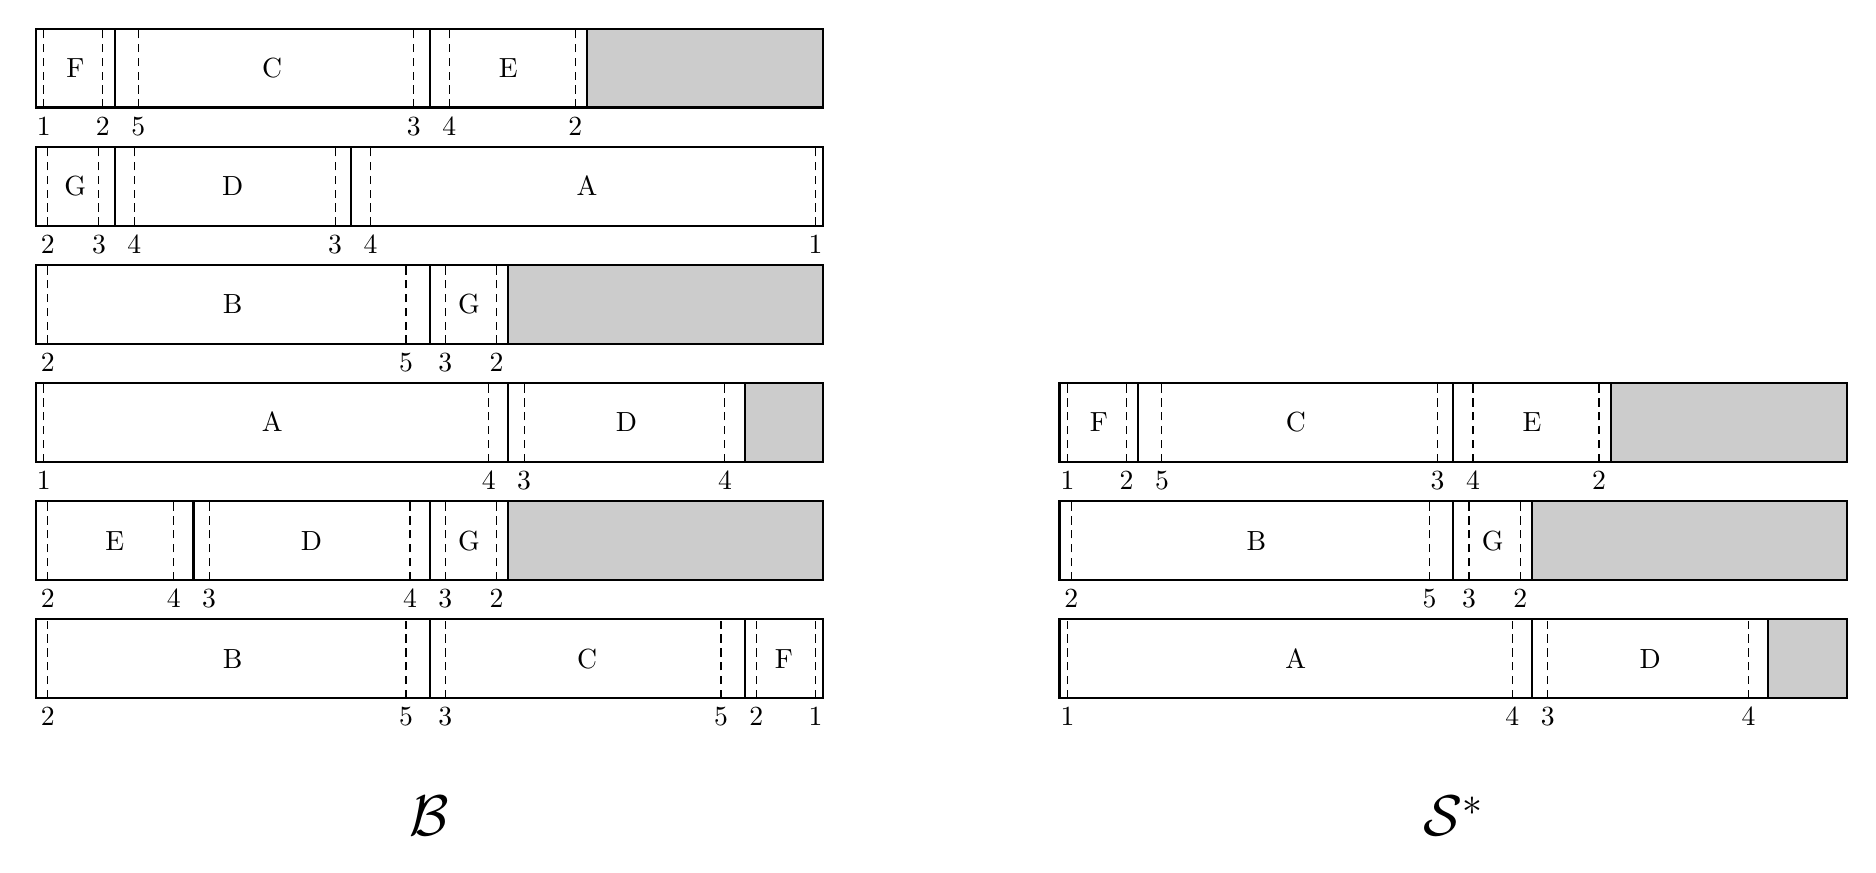
\begin{tikzpicture}
%\draw [help lines] (-1,-2) grid (13,11);

%---------- SET B OF BINS ----------%

\node at (5, -1.5) {\huge{$\mathcal{B}$}};

% F, C, E (1,4,2) (1-2, 5-3, 4-2) - part of the exact cover solution
%\path [fill=tLightPink] (0,7.5) rectangle (9.9,8.5);
\draw [thick] (0,7.5) rectangle (10, 8.5);
\draw [thick] (1,7.5) -- (1, 8.5);
\draw [thick] (5,7.5) -- (5, 8.5);
\filldraw[fill=black!20!white, draw=black, thick] (7,7.5) rectangle (10,8.5);
\draw [densely dashed] (0.1,7.5) -- (0.1,8.5);
\draw [densely dashed] (0.85,7.5) -- (0.85,8.5);
\draw [densely dashed] (1.3,7.5) -- (1.3,8.5);
\draw [densely dashed] (4.8,7.5) -- (4.8,8.5);
\draw [densely dashed] (5.25,7.5) -- (5.25,8.5);
\draw [densely dashed] (6.85,7.5) -- (6.85,8.5);
\node at (0.5,8) {F};
\node at (3,8) {C};
\node at (6,8) {E};
\node [below] at (0.1,7.5) {1};
\node [below] at (0.85,7.5) {2};
\node [below] at (1.3,7.5) {5};
\node [below] at (4.8,7.5) {3};
\node [below] at (5.25,7.5) {4};
\node [below] at (6.85,7.5) {2};

% G, D, A (1,3,6) (2-3, 4-3, 4-1)
%\path [fill=tLightPink] (0,6) rectangle (9.51,7);
\draw [thick] (0,6) rectangle (10, 7);
\draw [thick] (1,6) -- (1,7);
\draw [thick] (4,6) -- (4,7);
%\filldraw[fill=black!20!white, draw=black, thick] (9.51,6) rectangle (10,7);
\draw [densely dashed] (0.15,6) -- (0.15,7);
\draw [densely dashed] (0.8,6) -- (0.8,7);
\draw [densely dashed] (1.25,6) -- (1.25,7);
\draw [densely dashed] (3.8,6) -- (3.8,7);
\draw [densely dashed] (4.25,6) -- (4.25,7);
\draw [densely dashed] (9.9,6) -- (9.9,7);
\node at (0.5,6.5) {G};
\node at (2.5,6.5) {D};
\node at (7,6.5) {A};
\node [below] at (0.15,6) {2};
\node [below] at (0.8,6) {3};
\node [below] at (1.25,6) {4};
\node [below] at (3.8,6) {3};
\node [below] at (4.25,6) {4};
\node [below] at (9.9,6) {1};


% B, G (5,1) (2-5, 3-2) - part of the exact cover solution
%\path [fill=tLightPink] (0,4.5) rectangle (8.89,5.5);
\draw [thick] (0,4.5) rectangle (10, 5.5);
\draw [thick] (5,4.5) -- (5,5.5);
\filldraw[fill=black!20!white, draw=black, thick] (6,4.5) rectangle (10,5.5);
\draw [densely dashed] (0.15,4.5) -- (0.15,5.5);
\draw [densely dashed] (4.7,4.5) -- (4.7,5.5);
\draw [densely dashed] (5.2,4.5) -- (5.2,5.5);
\draw [densely dashed] (5.85,4.5) -- (5.85,5.5);
\node at (2.5,5) {B};
\node at (5.5,5) {G};
\node [below] at (0.15,4.5) {2};
\node [below] at (4.7,4.5) {5};
\node [below] at (5.2,4.5) {3};
\node [below] at (5.85,4.5) {2};


% A, D (6, 3) (1-4, 3-4) - part of the exact cover solution
%\path [fill=tLightPink] (0,3) rectangle (7.49,4);
\draw [thick] (0,3) rectangle (10, 4);
\draw [thick] (6,3) -- (6,4);
\filldraw[fill=black!20!white, draw=black, thick] (9,3) rectangle (10,4);
\draw [densely dashed] (0.1,3) -- (0.1,4);
\draw [densely dashed] (5.75,3) -- (5.75,4);
\draw [densely dashed] (6.2,3) -- (6.2,4);
\draw [densely dashed] (8.75,3) -- (8.75,4);
\node at (3,3.5) {A};
\node at (7.5,3.5) {D};
\node [below] at (0.1,3) {1};
\node [below] at (5.75,3) {4};
\node [below] at (6.2,3) {3};
\node [below] at (8.75,3) {4};


% E, D, G (2,3,1) (2-4, 3-4, 3-2)
%\path [fill=tLightPink] (0,1.5) rectangle (8.37,2.5);
\draw [thick] (0,1.5) rectangle (10, 2.5);
\draw [thick] (2,1.5) -- (2,2.5);
\draw [thick] (5,1.5) -- (5,2.5);
\filldraw[fill=black!20!white, draw=black, thick] (6,1.5) rectangle (10,2.5);
\draw [densely dashed] (0.15,1.5) -- (0.15,2.5);
\draw [densely dashed] (1.75,1.5) -- (1.75,2.5);
\draw [densely dashed] (2.2,1.5) -- (2.2,2.5);
\draw [densely dashed] (4.75,1.5) -- (4.75,2.5);
\draw [densely dashed] (5.2,1.5) -- (5.2,2.5);
\draw [densely dashed] (5.85,1.5) -- (5.85,2.5);
\node at (1,2) {E};
\node at (3.5,2) {D};
\node at (5.5,2) {G};
\node [below] at (0.15,1.5) {2};
\node [below] at (1.75,1.5) {4};
\node [below] at (2.2,1.5) {3};
\node [below] at (4.75,1.5) {4};
\node [below] at (5.2,1.5) {3};
\node [below] at (5.85,1.5) {2};


% B, C, F (5,4,1) (2-5, 3-5, 2-1)
%\path [fill=tLightPink] (0,0) rectangle (8.52,1);
\draw [thick] (0,0) rectangle (10, 1);
\draw [thick] (5,0) -- (5,1);
\draw [thick] (9,0) -- (9,1);
%\filldraw[fill=black!20!white, draw=black, thick] (6,0) rectangle (10,1);
\draw [densely dashed] (0.15,0) -- (0.15,1);
\draw [densely dashed] (4.7,0) -- (4.7,1);
\draw [densely dashed] (5.2,0) -- (5.2,1);
\draw [densely dashed] (8.7,0) -- (8.7,1);
\draw [densely dashed] (9.15,0) -- (9.15,1);
\draw [densely dashed] (9.9,0) -- (9.9,1);
\node at (2.5,0.5) {B};
\node at (7,0.5) {C};
\node at (9.5,0.5) {F};
\node [below] at (0.15,0) {2};
\node [below] at (4.7,0) {5};
\node [below] at (5.2,0) {3};
\node [below] at (8.7,0) {5};
\node [below] at (9.15,0) {2};
\node [below] at (9.9,0) {1};


%-------------------------------------------------------

%---------- BINS IN EXACT COVER ----------%

\node at (18, -1.5) {\huge{$\mathcal{S}^*$}};

% F, C, E (1,4,2) (1-2, 5-3, 4-2) - part of the exact cover solution
\draw [thick] (13,3) rectangle (23, 4);
\draw [thick] (14,3) -- (14, 4);
\draw [thick] (18,3) -- (18, 4);
\filldraw[fill=black!20!white, draw=black, thick] (20,3) rectangle (23,4);
\draw [densely dashed] (13.1,3) -- (13.1,4);
\draw [densely dashed] (13.85,3) -- (13.85,4);
\draw [densely dashed] (14.3,3) -- (14.3,4);
\draw [densely dashed] (17.8,3) -- (17.8,4);
\draw [densely dashed] (18.25,3) -- (18.25,4);
\draw [densely dashed] (19.85,3) -- (19.85,4);
\node at (13.5,3.5) {F};
\node at (16,3.5) {C};
\node at (19,3.5) {E};
\node [below] at (13.1,3) {1};
\node [below] at (13.85,3) {2};
\node [below] at (14.3,3) {5};
\node [below] at (17.8,3) {3};
\node [below] at (18.25,3) {4};
\node [below] at (19.85,3) {2};


% B, G (5,1) (2-5, 3-2) - part of the exact cover solution
\draw [thick] (13,1.5) rectangle (23, 2.5);
\draw [thick] (18,1.5) -- (18,2.5);
\filldraw[fill=black!20!white, draw=black, thick] (19,1.5) rectangle (23,2.5);
\draw [densely dashed] (13.15,1.5) -- (13.15,2.5);
\draw [densely dashed] (17.7,1.5) -- (17.7,2.5);
\draw [densely dashed] (18.2,1.5) -- (18.2,2.5);
\draw [densely dashed] (18.85,1.5) -- (18.85,2.5);
\node at (15.5,2) {B};
\node at (18.5,2) {G};
\node [below] at (13.15,1.5) {2};
\node [below] at (17.7,1.5) {5};
\node [below] at (18.2,1.5) {3};
\node [below] at (18.85,1.5) {2};


% A, D (6, 3) (1-4, 3-4) - part of the exact cover solution
\draw [thick] (13,0) rectangle (23, 1);
\draw [thick] (19,0) -- (19,1);
\filldraw[fill=black!20!white, draw=black, thick] (22,0) rectangle (23,1);
\draw [densely dashed] (13.1,0) -- (13.1,1);
\draw [densely dashed] (18.75,0) -- (18.75,1);
\draw [densely dashed] (19.2,0) -- (19.2,1);
\draw [densely dashed] (21.75,0) -- (21.75,1);
\node at (16,0.5) {A};
\node at (20.5,0.5) {D};
\node [below] at (13.1,0) {1};
\node [below] at (18.75,0) {4};
\node [below] at (19.2,0) {3};
\node [below] at (21.75,0) {4};





\end{tikzpicture}
	
\end{document}